\chapter{Simulation and Event Reconstruction for the ATLAS Experiment}

In current LHC pp collison, bunches of protons collide every 25 nanoseconds (ns), which gives a large challenge to event reconstruction and selections.
To predict and model each process, the Monte Carlo simulations of physics events are essential for high-energy physics experiments.
This section will briefly discuss the event simulation and reconstruction programs based on the ATLAS software framework. 

\section{Event sumilation}
%\subsection{Simulation framework}

The ATLAS simulation program is integrated into the ATLAS software framework called \textit{Athena}~\cite{atlas:athena},
which uses Python as an object-oriented scripting and interpreter language to configure and load C++ algorithms and objects.
Figure~\ref{fig:frame_overview} shows the overview of ATLAS simulation data flow~\cite{Aad:2010ah}.
In the diagrams, the square-cornered boxes represents algorithms and applications to be run and round-cornered boxes denote data objects.
\begin{figure}[!htb]
  \centering
  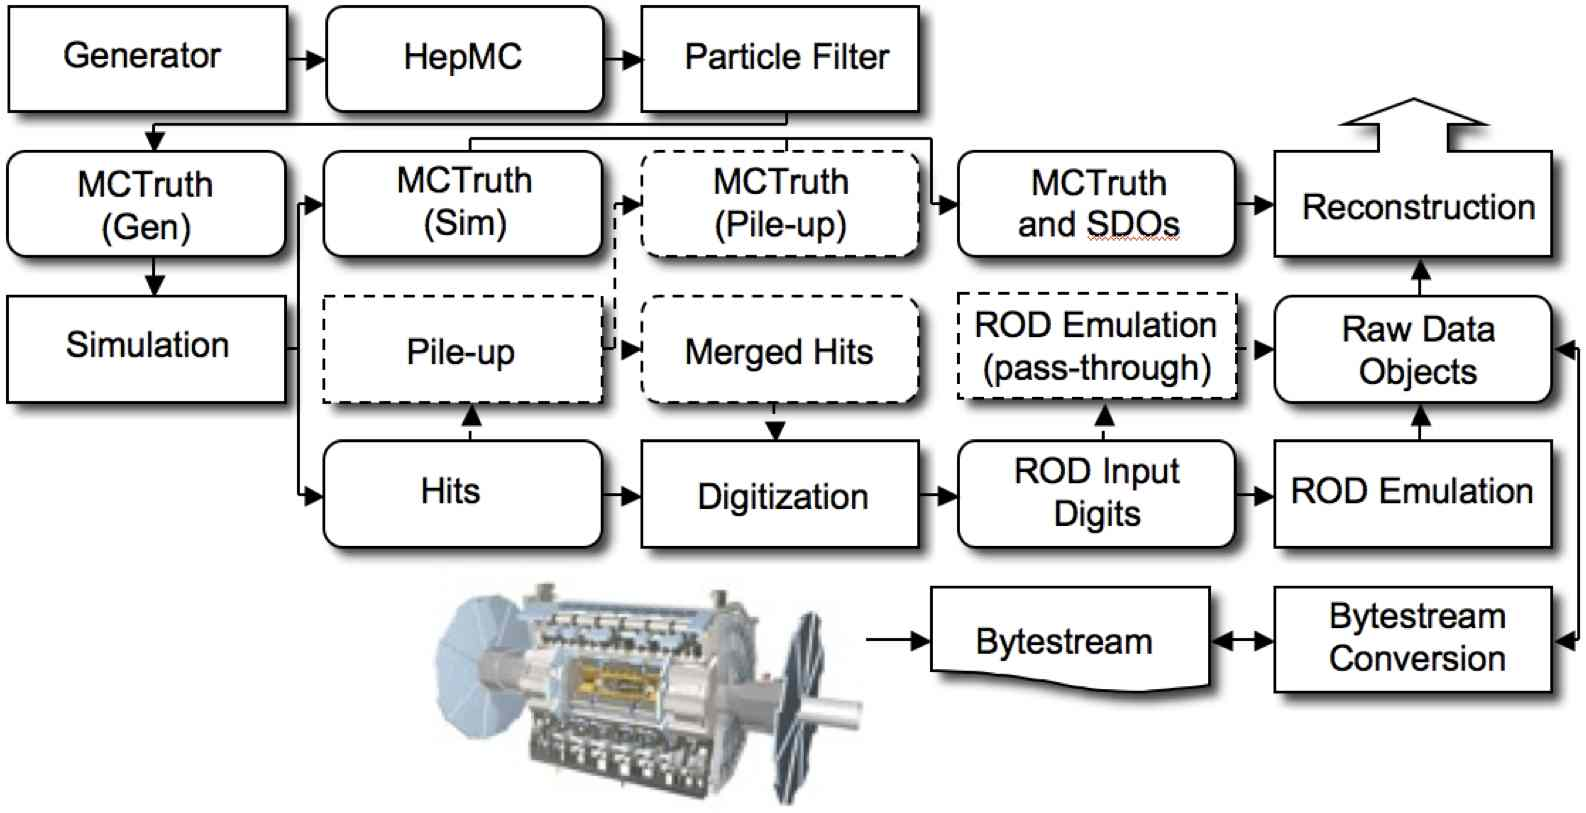
\includegraphics[width=1.0\textwidth]{figures/Simulation/outline_atalsSimulation_v2.png}
  \caption{The flow of the ATLAS simulation software.}
  \label{fig:frame_overview}
\end{figure}

First of all, events are produced by MC generators in standard HepMC format and then read into the simulation.
During the simulation, particles are propagated through the full ATLAS detector whose configurations can be set by users via GEANT4 toolkit.
The energies deposited in the sensitive regions of the detector are recorded as \textit{hits} that contains the total energy deposition,
position and time, and are written to a simulation hit file.
In the meatime, the events in "truth" format are also recorded to contain the history of the interactions from the generator, including incoming and outgoing particles.
Simulated Data Objects (SDOs) are created from truth, which are maps between hits in sensitive portions of the detector and truth information of particles in simulation.
The files are then sent to digitization, with constructs ``digits" inputs and be written into Raw Data Object (RDO) file used for reconstruction.

In conclusion, there are three main parts of framework: \textit{Generation}, \textit{Simulation} and \textit{Digitization}.
More details are given as below:

\textbf{Event generation}

As shown in figure~\ref{fig:mc_event_structure}~\cite{Hoche:2014rga}, at hardon colliders, multiple scattering and rescattering effects arise, which needs to be simulated by Monte Carlo (MC) event generators to reflect the full complexity of those event structures.
Several MC event generators can be used to generate events originally in HepMC format.
The events can be filtered at generation time with some certain requirements (eg. decay channel or missing energy above a certain threshold).
The generator is responsible for any prompt decays (e.g. W or Z bosons) but stores any "stable" particle expected to propagate through a part of the detector. 
During the generation steps, any interactions with detector are ignored and only immediate decays are considered.

There are several MC generators that have been widely used with general purpose, which include \textsc{Sherpa}~\cite{Gleisberg_2009}, \textsc{Herwig++}~\cite{Bahr2008}, \textsc{PowhegBox}~\cite{Nason:2004rx}, \textsc{MC@NLO}~\cite{Frixione_2002} and \textsc{Pythia8}~\cite{Sjostrand:2007gs}.

\begin{figure}[!htb]
  \centering
  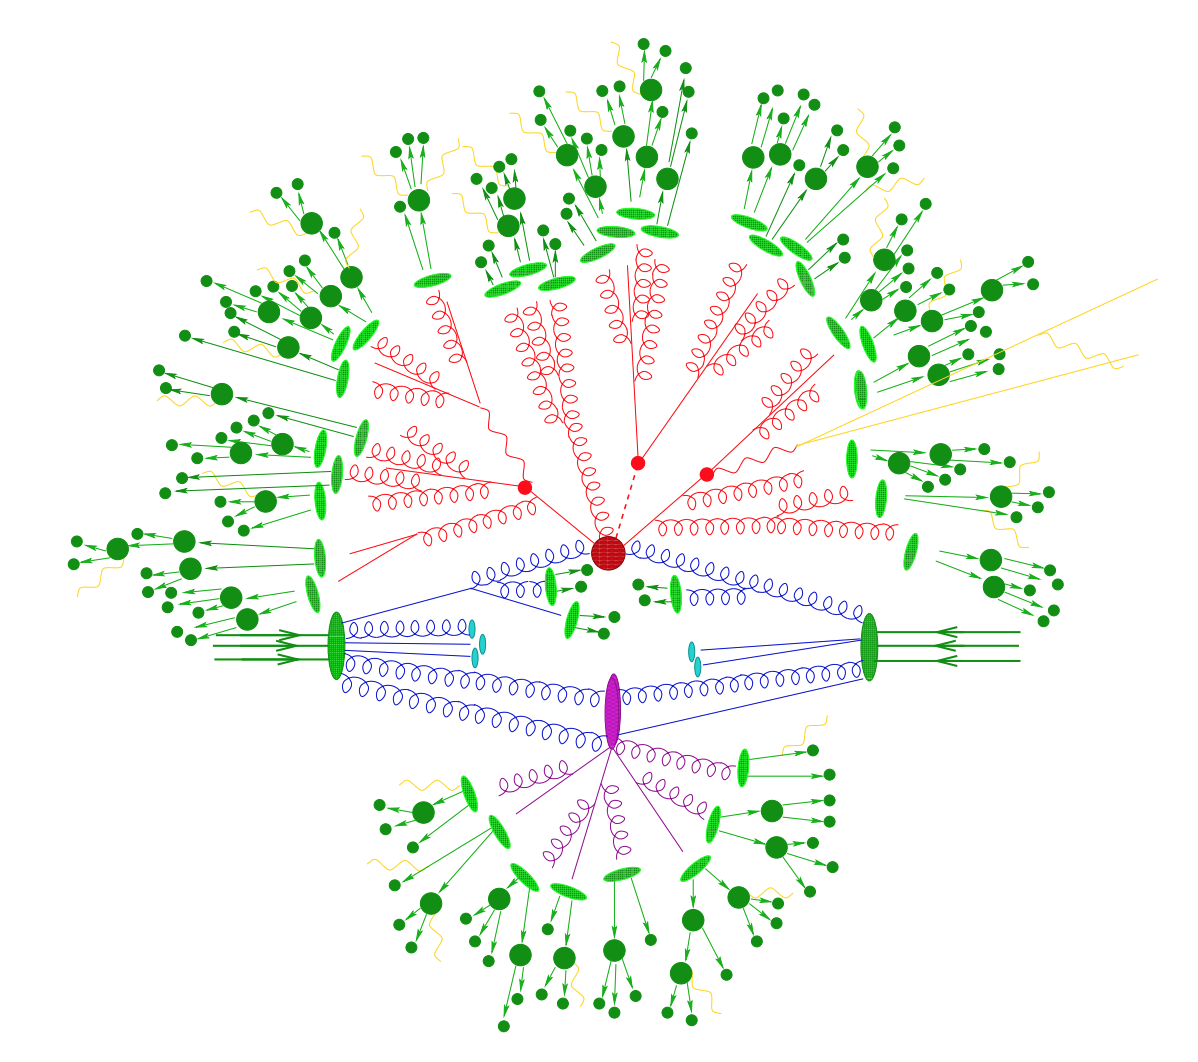
\includegraphics[width=0.7\textwidth]{figures/Simulation/mc_event_structure.png}
  \caption{Sketch of a hardon-hardon collision simulated by MC event generator. The red blob in center denotes the hard collision, surrounded by tree-like structures representing Bremsstrahlung which is simulated by Parton Showers. The purple blob stands for a secondary hard scattering event. The light green blobs indecate the parton-to-hardon transitions and the dark green blobs represents hardon decays. The yellow lines are soft photon radiations.}
  \label{fig:mc_event_structure}
\end{figure}

\textbf{Simulation}

GEANT4 is used as standard simulation toolkit for the ATLAS experiment, which transports physics particles through the detector's geometry.
During the generation level, the entire connected chain of the HepMC event is stored as the Monte Carlo truth. 
Only the stable particles are read into GEANT4 for further simulation and selection, while transformations can be applied to these events to select certain processes.
During the simulation, many secondary tracks can be produced, therefore only information from the interactions of interest are stored, including the incoming particles, step sequence, vertex as well as outgoing particles.
The output of GEANT4 is called \textit{hit file}, which contains metadata describing the configuration of the simulation during the run, all truth information requested and a collection of hits for each subdetector.

Since the standard ATLAS detector simulation cost very large computing resources to accurately model the complex detector geometry and physics descriptions, some fast simulation programss are developed according to different user purpose.
Some popular fast-sim toolkits include \textit{Fast G4 Simulation}~\cite{Barberio:2007gba}, \textit{ATLFAST-I}~\cite{Richter-Was:683751} and \textit{ATLFAST-II}~\cite{Edmonds:1091969}.

\textbf{Digitization}

The hit outputs from simulated events, including hard scattering signal, minimum bias, beam halo, beam gas and cavern background events, are then sent into digitization procedure, converted into detector response called ``digits".
Before converted into detector signal as `digits' formart, each type of event can be overlaid at a user-specified rate.
Those overlay, called ``pile-up", can be done during degitization to save the CPU time.
At this stage, the detector noise and the first level trigger that implemented with hardware on the real detector are added into events.
The digitization firstly constructs ``digits" inputs to the readout drivers (RODs) in the detector electronics.
Then the ROD functionality is emulated, and the output digits are written out as Raw Data Object (RDO) file.
In addition, the digitization algorithms can also produce Simulated Data Objects (SDOs), which contain information about all the particles, noise and the amount of energy that contributed to the signal. 
Then all information are sent into reconstruction level described in next subsection.

%\subsection{Simulation framework}

\subsection{Event reconstruction}

The data flow of ATLAS data processing is sketched in figure~\ref{fig:data_processing}\cite{Boyd_2010}. 
Data from detector is firstly filtered by online trigger system and then send to the \textit{Tier-0 (T0)} for initial processing by offline reconstruction software also based on Athena.
A small amount of data named "express stream" is processed in almost real time in T0 for online data quality monitoring.
In addition, some other dedicated data steams are sent out at trigger level for detector alignment and calibration.
These calibration and alignment information are then used for bulk reconstruction in T0.
At the end of the reconstruction chain, the data are delivered into \textit{Tier-1 (T1)} and \textit{Tier-2 (T2)} centers for further analysis and production of simulated data.
Besides, T1 centers are also responsible for data reprocessing by re-running data reconstruction with improved calibration and alignment constants and with improved reconstruction algorithms.
This sub-section describes the reconstruction of some important physics objects in ATLAS experiment, i.e. tracks, vertices, electrons, muons, jets, and missing energies.
\begin{figure}[!htb]
  \centering
  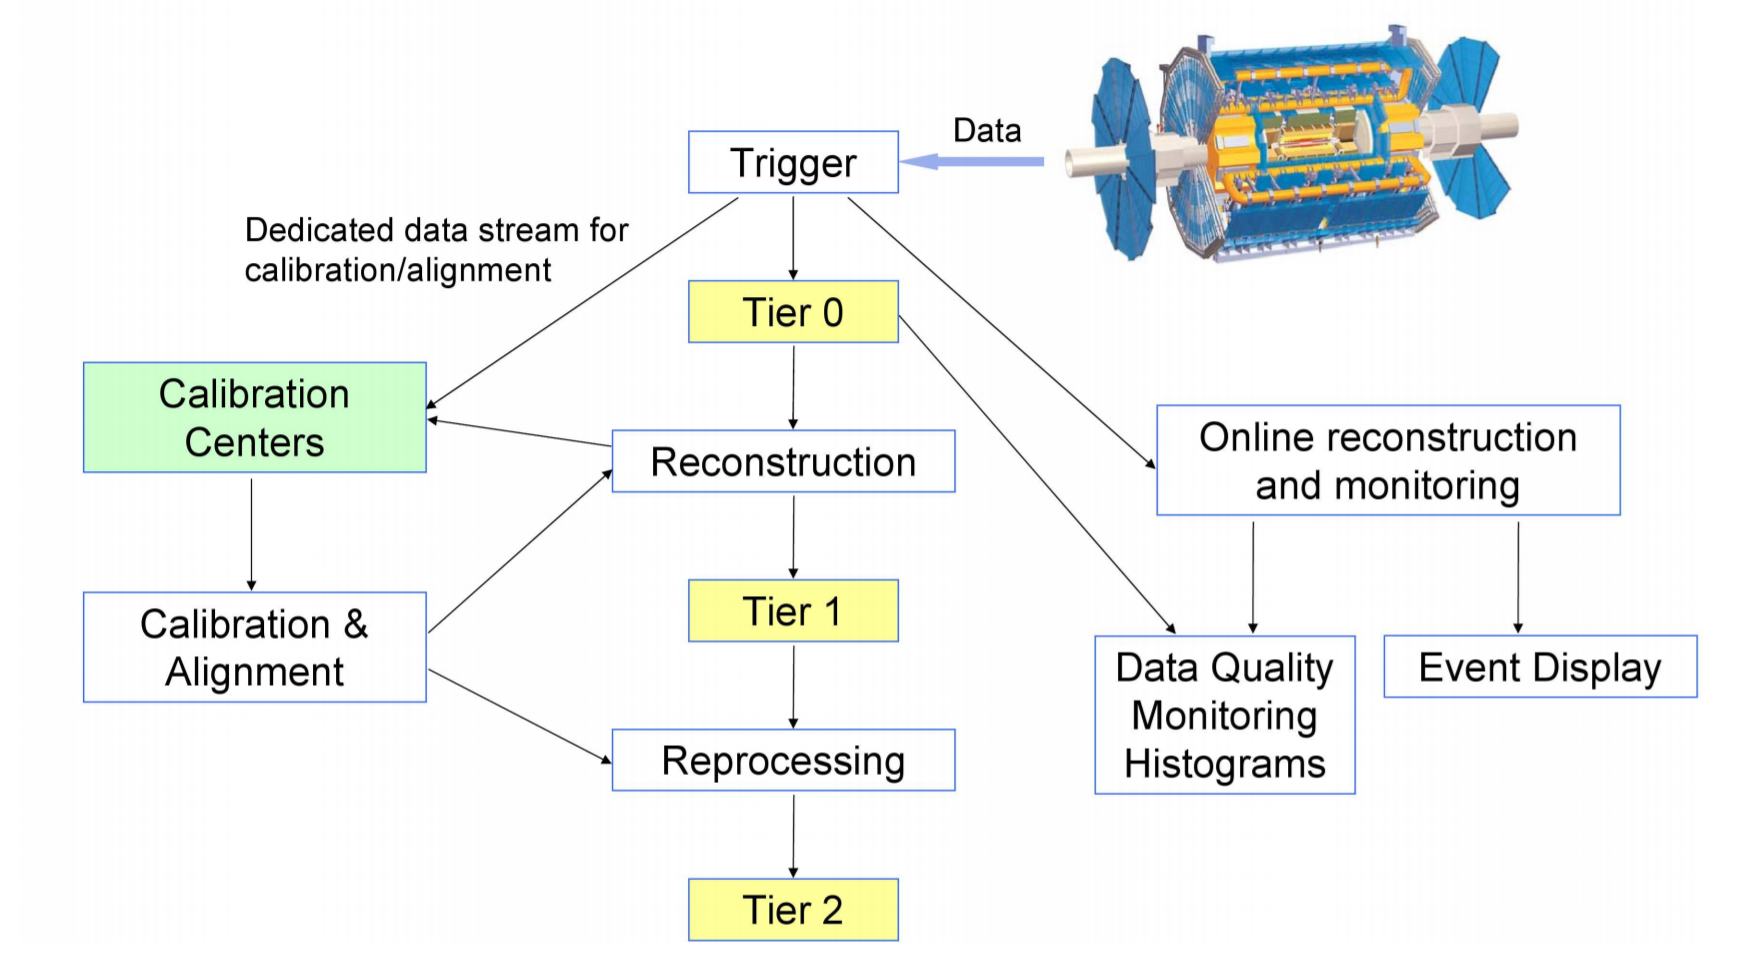
\includegraphics[width=0.9\textwidth]{figures/Simulation/data_processing.png}
  \caption{The flowchart of the ATLAS data processing.}
  \label{fig:data_processing}
\end{figure}

\subsection{Track}
\label{sec:track}

The ATLAS detector is composed of two independent tracking systems: the Inner Detector (ID) close to the interaction point, and the Muon Spectrometer (MS) located in the outermost region.
The reconstructed charged-particle trajectories in the ID and MS are referred to as ID tracks and MS tracks respectively.
The challenge of ID reconstruction is that it needs to handle high track density that imposes a large number of combinatorial track candidates, 
while the MS reconstruction is however largely limited by the huge amount of inert material, the large background and the highly inhomogeneous magnetic field~\cite{Cornelissen:1020106}.
More details of these two types of track are given as below:

\textbf{Inner detector track}

Figure~\ref{fig:track_ID} sketches the ID system used for detecting charge-particle tracks.
The ID track reconstructions contains two sequences: \textit{inside-out} track reconstruction and \textit{outside-in} one.
\begin{figure}[!htb]
  \centering
  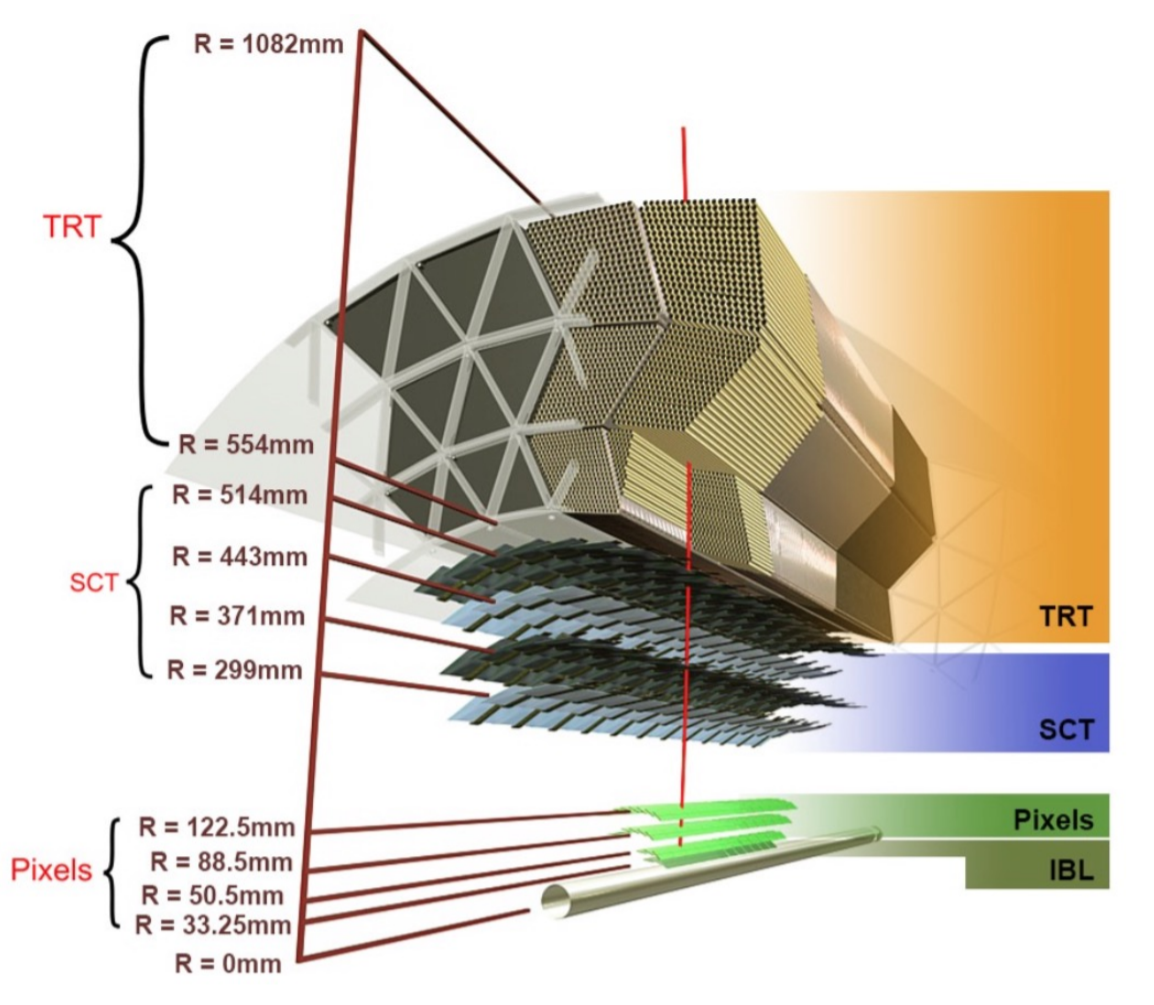
\includegraphics[width=0.7\textwidth]{figures/Simulation/track_ID.png}
  \caption{Schematic view of the ATLAS inner detector showing all the corresponding components.}
  \label{fig:track_ID}
\end{figure}

For inside-out tracking, it exploits the high granularity of the pixel and SCT detectors to discover prompt tracks originating from the interaction point.
In first step, the track seeds are formed by combining the information of space-points in the three pixel layers and the first SCT layer.
Then, these seeds are extended throughout the SCT to build track candidates.
After that, these candidates are fitted with some quality cuts applied to remove the outlier clusters, reject the fake tracks and resolve ambiguities in the cluster-to-track association.
The selected tracks are then further extended to TRT, and refitted with the full information from pixel, SCT and TRT detectors.

Another complementary approach, outside-in, searches for unused track segments start from TRT instead.
These segments are then extended into the SCT and pixel detectors to improve the tracking efficiency for secondary tracks from conversions or decays of long-lived particles.

\textbf{Muon spectrometer track}

The MS track reconstruction\cite{Aad:2016jkr} starts from searching hit patterns inside each muon chamber to form segments.
In each MDT chamber and nearby trigger chamber, a Hough transform\cite{ILLINGWORTH198887} is used to search the hits lie on a certain trajectory in the bending plane of the detector.
The MDT segments are reconstructed by performing a linear fit to the hits found in each layer.
The RPC or TGC hits can be built by measuring the coordinate orthogonal to the bending plane.
And the segments of CSC can be built using a separate combinatorial search in the $\eta$ and $\phi$ detector planes.

Then muon track candidates are built by fitting hits from segments in different layers together.
This task makes use of the algorithm by performing a segment-seeded combinatorial search, which starts by using the segments generated in the middle layers of the detector where more trigger hits are available as seeds.
The search is then extended to use the segments as seeds from the inner and outer layers.
The segments are selected based on criteria of hit multiplicity and fit quality, and are matched using their relative positions and angles.
To build a track, at least two matching segments are required, except in the barrel-endcap transition region where a single high-quality segment with $\eta$ and $\phi$ information can be used to build a track.
At beginning, the same segment can be used to build more than one track candidates.
Later on, an overlap removal algorithm is performed to select the best assignment to a single track, or decide whether allows the certain segment to be shared between two tracks.

The hits associated with each track candidate are then fitted using a global $\chi^{2}$ fit.
The algorithm accepts the track candidate if its fitting $\chi^{2}$ passes the selection criteria.
Hits contribute largely to $\chi^{2}$ are removed and the track fit is repeated.
In addition, the algorithm performs a hit recovery procedure that looks for additional hits consistent with the candidate trajectory, and the track candidate is refit if additional hits are found.

